\documentclass[12pt]{article}

\usepackage[utf8]{inputenc}
\usepackage{geometry}

\usepackage{graphicx} 

%%% PACKAGES
\usepackage{booktabs} 
\usepackage{array} 
\usepackage{paralist} 
\usepackage{verbatim} 
\usepackage{subfig} 
\usepackage{hyperref}
%%% HEADERS & FOOTERS
\usepackage{fancyhdr} % This should be set AFTER setting up the page geometry
%%% SECTION TITLE APPEARANCE
\usepackage{sectsty}
%%% ToC (table of contents) APPEARANCE
\usepackage[nottoc,notlof,notlot]{tocbibind} % Put the bibliography in the ToC
\usepackage[titles,subfigure]{tocloft} % Alter the style of the Table of Contents
%%% For code listing
\usepackage{listings} % Gives syntax highlighting for python code. 
\usepackage{color} % Used for syntax highlighting. 
\usepackage{textcomp} % Used for syntax highlighting. 
%%% SETTINGS
\geometry{letterpaper} 
\geometry{margin=0.75in}
\pagestyle{fancy} 
\renewcommand{\headrulewidth}{0.5pt} 
\lhead{}\chead{2012 Groundwater Workshop -- \texttt{matplotlib} Examples}\rhead{}
\lfoot{}\cfoot{\thepage}\rfoot{}
\allsectionsfont{\sffamily\mdseries\upshape} 
\renewcommand{\cftsecfont}{\rmfamily\mdseries\upshape}
\renewcommand{\cftsecpagefont}{\rmfamily\mdseries\upshape} 
%\captionsetup{labelformat=empty,labelsep=none}
% This gives syntax highlighting in the python environment 
\definecolor{gray}{gray}{0.5} 
\definecolor{key}{rgb}{0,0.5,0} 
\lstset{
basicstyle=\ttfamily\tiny, 
otherkeywords={ -, =, +, [, ], (, ), \{, \}, :, *, !}, 
keywordstyle=\color{blue}, 
stringstyle=\color{red},
showstringspaces=false,
alsoletter={1234567890},
otherkeywords={\ , \}, \{},
keywordstyle=\color{blue},
emph={access,and,break,class,continue,def,del,elif ,else,%
except,exec,finally,for,from,global,if,import,in,is,%
lambda,not,or,pass,print,raise,return,try,while},
emphstyle=\color{black}\bfseries,
emph={[2]True, False, None, self},
emphstyle=[2]\color{green},
emph={[3]from, import, as},
emphstyle=[3]\color{blue},
upquote=true,
morecomment=[s]{"""}{"""},
commentstyle=\color{gray}\slshape,
emphstyle=[4]\color{blue},
literate=*{:}{{\textcolor{blue}:}}{1}%
{=}{{\textcolor{blue}=}}{1}%
{-}{{\textcolor{blue}-}}{1}%
{+}{{\textcolor{blue}+}}{1}%
{*}{{\textcolor{blue}*}}{1}%
{!}{{\textcolor{blue}!}}{1}%
{(}{{\textcolor{blue}(}}{1}%
{)}{{\textcolor{blue})}}{1}%
{[}{{\textcolor{blue}[}}{1}%
{]}{{\textcolor{blue}]}}{1}%
{<}{{\textcolor{blue}<}}{1}%
{>}{{\textcolor{blue}>}}{1},%
numbers=none,
}
\newcommand{\putat}[3]{\begin{picture}(0,0)(0,0)\put(#1,#2){#3}\end{picture}}


\title{2012 USGS National Groundwater Workshop \\ Using \texttt{python} to Improve Groundwater \\ Model Effectiveness: A \\ \texttt{matplotlib} Example Problems}
\author{}
\date{August 9, 2012}

\begin{document}
\maketitle

\section{Getting started}
Open a command window and navigate to the MATPLOTLIB$\backslash$python subdirectory (\textbf{fig.~\ref{FigGettingStarted}}).

\begin{figure}
	\centering
  	\includegraphics[width=8.25cm]{figures/GettingStarted.png}
 	\caption{Getting started with the exercise.}
	\label{FigGettingStarted}
\end{figure}

\section{\texttt{matplotlib} exercise 1 -- create a simple plot}
Download discharge data from NWIS for ``USGS 06719505 CLEAR CREEK AT GOLDEN, CO'' for the period from 8/1/2011 to 8/1/2012 and save as a space delimited file containing only the date and discharge data in the MATPLOTLIB$\backslash$data subdirectory (a suggested name is \texttt{ClearCreek.txt}). If you do not have internet access, a prepared file is available (\texttt{06719505.txt}) in the MATPLOTLIB$\backslash$data subdirectory. Create a new python script in the MATPLOTLIB$\backslash$python subdirectory (a suggested name is \texttt{Ex1.py}). Open the python script you created in a text editor.

\subsection{Read the Clear Creek data}
Import the necessary datetime, pylab, numpy, and matplotlib modules and read the discharge data by adding the following to your blank python file (\texttt{Ex1.py}).

\begin{center}
	\lstinputlisting[language=python,firstline=1,lastline=7]{data/Ex1.py}
\end{center}

Depending on the date format you used when saving \texttt{ClearCreek.txt} \texttt{python} may experience some difficulty parsing the date. If this occurs, modify \texttt{dt.datetime} to \texttt{`|S10'} in the \texttt{dtype=} statement in \texttt{np.genfromtext}. To create a basic plot and print to the screen add the following lines to your python file. 

\begin{center}
	\lstinputlisting[language=python,firstline=8,lastline=13]{data/Ex1.py}
\end{center}

Run the script from the command line (\textbf{fig.~\ref{FigGettingStarted}}) by typing \texttt{python Ex1.py} and pressing enter. You should see the graphic shown in \textbf{figure~\ref{FigEx1ScreenPlot}} if the script executes correctly.

\begin{figure}
	\centering
  	\includegraphics[height=3in]{figures/pl_PLOT.png}
 	\caption{\texttt{matplotlib} exercise 1 screen output.}
	\label{FigEx1ScreenPlot}
\end{figure}

\subsection{Modifying the axes and adding labels}
Add the following lines to modify the extent of the x-axis and add labels to the x- and y-axes.

\begin{center}
	\lstinputlisting[language=python,firstline=15,lastline=17]{data/Ex1.py}
\end{center}

These lines should be added before the \texttt{pl.show()} command. The \texttt{r} prior to the string in the \texttt{pl.ylabel} command allows \LaTeX \hspace{1pt} equations and equation formatting to be embedded in strings shown in the plot. The x-axis is limited to be between 0 and 365 using the \texttt{xlim} command because there are only 366 days in the dataset for Clear Creek (remember \texttt{python} is zero-based). After saving these modifications rerun the script. You should see the graphic shown in  \textbf{figure~\ref{FigEx1ModScreenPlot}} if the modified script executes correctly.

\begin{figure}
	\centering
  	\includegraphics[height=3in]{figures/pl_PLOT_axes.png}
 	\caption{\texttt{matplotlib} exercise 1 screen output with axes modifications.}
	\label{FigEx1ModScreenPlot}
\end{figure}

\subsection{Saving the plot as an image}
To save the plot to an image file modify the script by commenting out the \texttt{pl.show()} command and adding the \texttt{pl.savefig} command as shown below. The resulting figure is shown \textbf{figure~\ref{FigEx1Export}}.

\begin{center}
	\lstinputlisting[language=python,firstline=19,lastline=22]{data/Ex1.py}
\end{center}

\begin{figure}[hp]
	\centering
  	\includegraphics[height=3in]{../figures/matplotlibExercise1-base.png}
 	\caption{\texttt{matplotlib} exercise 1 exported image file.}
	\label{FigEx1Export}
\end{figure}

\subsection{Additional tasks}
Some additional tasks that you can attempt if you have time are changing the color, line weight, line style, \textit{etc.} of the Clear Creek discharge data. You should refer to \url{http://matplotlib.sourceforge.net/api/pyplot_api.html\#matplotlib.pyplot.plot} for guidance on modifying these (and other) options.

\section{\texttt{matplotlib} exercise 2 -- working with subplots}
A base \texttt{python} script for exercise 2 (\texttt{BarChartBase.py}) has been provided. Make a copy of this file so you can backtrack in the event that you make and error and need to start over; a suggested sript name is \texttt{Ex2.py}.

\subsection{Getting started with subplots}
In this exercise we are going to read some meteorologic data (\texttt{data$backslash$MeterologicData.csv}) and plot multiple plots on a single \texttt{matplotlib} figure. The portion of the python script that reads and processes the data is shown below. The \texttt{np.genfromtxt} is quite complicated the primary task that this command is performing is parsing \texttt{datetime} data and filling missing data values. The data file \texttt{data$\backslash$MeterologicData.csv} contains rainfall, potential evapotranspiration (PET), minimum air temperature, and maximum air temperature. The script also includes logic for calculating monthly rainfall and PET.

\begin{center}
	\lstinputlisting[language=python,firstline=26,lastline=49]{data/Ex2.py}
\end{center}

The \texttt{add\_subplot(row,col,subplot)} command is used to create subplots in a \texttt{matplotlib} figure. The same \texttt{matplotlib} commands are used to create and format the subplot as is used for single plot \texttt{matplotlib} figures.

\begin{center}
	\lstinputlisting[language=python,firstline=62,lastline=83]{data/Ex2.py}
\end{center}

This script plots air temperature on the first subplot using a line graph (using the \texttt{plot} command) and monthly rainfall on the second subplot using a bar chart (using the \texttt{bar} command). The command \texttt{pl.date2num(d[`date'])} converts the \texttt{datetime} data to a number format that can be plotted by \texttt{matplotlib}. Because we are working with \texttt{datetime} there are some commands for using dates on the x-axis. Please take some time to review the file before you begin modifying it. Prior to making any modifications to your file run the script which will create an output image named \texttt{figures$\backslash$Ex2.png} (\textbf{fig.~\ref{FigEx2Base}}).  

\begin{figure}[hp]
	\centering
  	\includegraphics[clip=true,trim=0in 1.5in 0in 0in,width=0.75\textwidth]{../figures/Ex2.png}
 	\caption{\texttt{matplotlib} exercise 2 initial figure output.}
	\label{FigEx2Base}
\end{figure}

\subsection{Add a third subplot}
What you are going to be doing is adding a third subplot and plotting monthly PET on a bar chart. The easiest thing to do is copy and paste the code for the second subplot and modifying it to plot the PET data. Your modifications should look something like the code listed below.

\begin{center}
	\lstinputlisting[language=python,firstline=93,lastline=103]{data/Ex2.py}
\end{center}

After saving and running the revised script the output image should look similar to \textbf{figure~\ref{FigEx2Step1}}.

\begin{figure}[hp]
	\centering
  	\includegraphics[width=0.75\textwidth]{figures/MeterologicBar_step1.png}
 	\caption{\texttt{matplotlib} exercise 2 figure output with the third subplot.}
	\label{FigEx2Step1}
\end{figure}

\subsection{Add a second axis to the second subplot}
It is relatively easy to add a second axis to individual subplots using the \texttt{twinx()} command. You will be adding a second axis to the second subplot showing the cumulative rainfall. Add the following to your script.

\begin{center}
	\lstinputlisting[language=python,firstline=106,lastline=107]{data/Ex2.py}
\end{center}

These two lines should be added immediately after the \texttt{ax.bar} command. The second axis label can be added by adding the following line after the \texttt{ax.set\_ylabel} command.

\begin{center}
	\lstinputlisting[language=python,firstline=109,lastline=109]{data/Ex2.py}
\end{center}

The resulting image should look similar to \textbf{figure~\ref{FigEx2Step2}}

\begin{figure}[hp]
	\centering
  	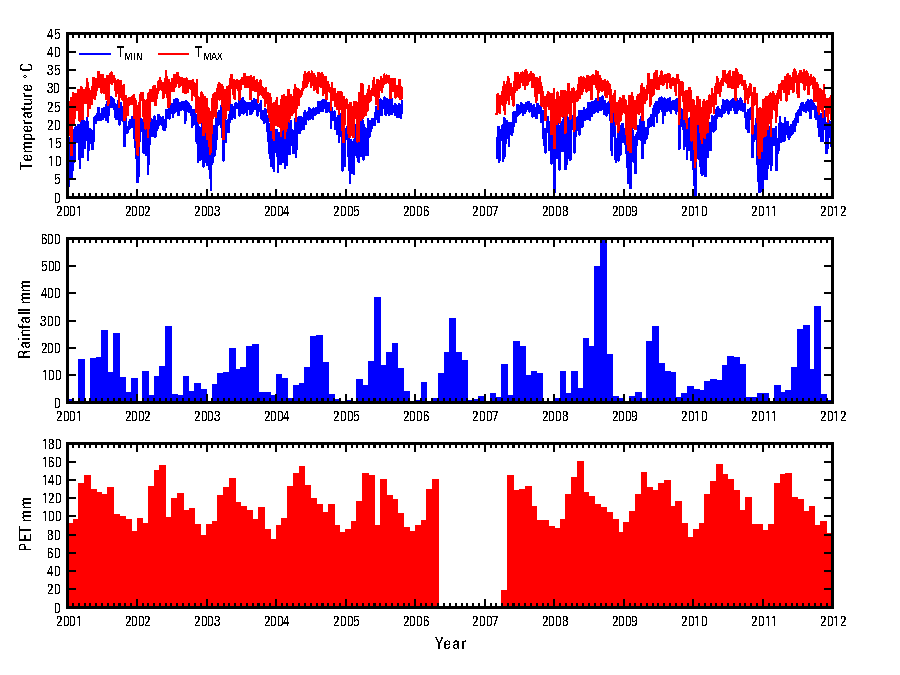
\includegraphics[width=0.75\textwidth]{../figures/MeterologicBar.png}
 	\caption{\texttt{matplotlib} exercise 2 figure output with the third subplot and a second axis on the second subplot.}
	\label{FigEx2Step2}
\end{figure}

\subsection{Additional tasks}
Some additional tasks that you can attempt if you have time are changing the colors, line weights, line styles, \textit{etc.} on any of the subplots. You should refer to \url{http://matplotlib.sourceforge.net/api/pyplot_api.html\#matplotlib.pyplot.plot} and \url{http://matplotlib.sourceforge.net/api/pyplot_api.html\#matplotlib.pyplot.bar} for guidance on modifying these (and other) options.

\section{\texttt{matplotlib} exercise 3 -- working with MODFLOW output}
A base \texttt{python} script for exercise 3 (\texttt{MODFLOWBase.py}) has been provided. Make a copy of this file so you can backtrack in the event that you make and error and need to start over; a suggested sript name is \texttt{Ex3.py}.

\subsection{Getting started with MODFLOW output}
Text

\end{document}
